\newpage
\section{Abstract}
    The report delves into strategies to tackle excessive meetings in project management, stressing structured and purposeful scheduling. Key recommendations encompass clear objectives, optimal frequency and duration, well-organized meetings, and participant perspectives. It advocates for special-purpose meetings, setting ground rules, and regular review for cancellation. Implementing these strategies enhances meeting efficiency, improving project outcomes and team satisfaction.
\section{Introduction}
Meetings are an integral part of project management and organizational communication. However, the prevalence of excessive and unproductive meetings has become a common complaint in many workplaces. To address this issue, it is essential to establish effective strategies for structuring, running, and eliminating unnecessary meetings. This report aims to provide comprehensive insights into the best practices for meeting management, with a focus on optimizing the structure and purpose of meetings, ensuring efficient facilitation, and minimizing the occurrence of unnecessary meetings.
\begin{center}
    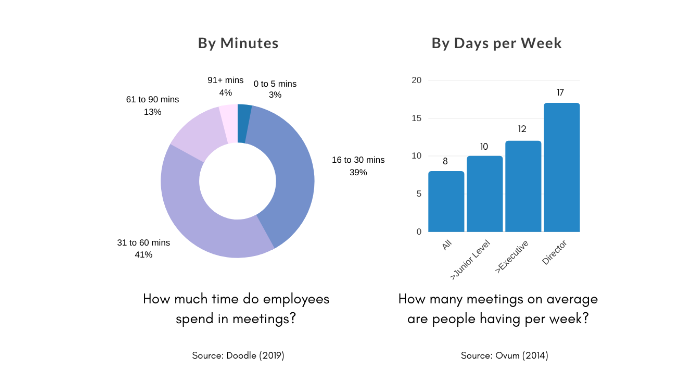
\includegraphics[width=150mm,height=80mm,scale=1]{TAS/Images/Meetings.png}\\ 
    {\bfseries Source: Minutes wasted of meetings statistics by }\href{https://www.booqed.com/blog/minutes-wasted-of-meeting-50-shocking-meeting-statistics}{BOOQED.com}
\end{center}
\subsection{Motivation}
The motivation for this report stems from the need to address the prevalent challenges associated with meeting management in project environments. The increasing dissatisfaction with excessive and unproductive meetings has led to a decline in productivity and employee engagement. This report aims to provide practical strategies for structuring, running, and eliminating unnecessary meetings to enhance project management efficiency and team productivity. The motivation is also inspired by the existing literature and discussions on the effects of team meetings on teams and organizational success ~\cite{01}. Meetings are an integral part of organizational life; however, few empirical studies have systematically examined the phenomenon and its effects on employees. By likening work meetings to interruptions and daily hassles, the authors proposed that meeting load ~\cite{05}.
In summary, the motivation for this report is driven by the necessity to address the challenges associated with meeting management, contribute to existing literature, and provide practical guidance for enhancing productivity and efficiency in project management.
\subsection{Problem Statement}
The problem lies in the inefficiency and ineffectiveness of meetings within project management and organizational settings. The prevalence of excessive, unproductive, and time-consuming meetings has led to decreased productivity, disengagement, and frustration among team members. The lack of clear guidelines for structuring and running meetings, as well as the failure to identify and eliminate unnecessary meetings, has contributed to this issue. Therefore, there is a critical need to address these challenges and establish effective meeting management practices to enhance productivity and engagement in the workplace.
\subsection{Objectives}
The investigation on minimizing meetings provides strategies for streamlined schedules, enhancing productivity, and addressing common complaints. By implementing recommended solutions, individuals and organizations can achieve better balance and improved efficiency, fostering job satisfaction through effective collaboration and focused work.
\begin{enumerate}
{\bfseries \item To Provide Effective Meeting Structuring Strategies}: This report aims to outline strategies for structuring meetings effectively, including the establishment of clear objectives, setting ground rules, and encouraging brevity ~\cite{04}.
{\bfseries \item  To Enhance Meeting Facilitation and Management}: The report seeks to provide insights into running meetings efficiently, including starting and ending meetings on time, utilizing a "bucket list" for off-topic issues, and summarizing decisions and outcomes after each meeting.
{\bfseries \item  To Minimize Unnecessary Meetings}: The report aims to offer guidance on identifying and eliminating unnecessary meetings, considering alternatives, and reviewing and canceling meetings that are not essential.\\
By addressing these objectives, the report endeavors to equip project leaders and meeting organizers with the knowledge and tools necessary to optimize meeting management, leading to increased productivity and efficiency in project management and organizational communication.
\end{enumerate}
\section{Literature Review}
\subsection{The Impact of Excessive Meetings}
Numerous studies highlight the adverse effects of too many meetings on organizational outcomes. A study by Allen and Rogelberg (2013) ~\cite{09} found a negative correlation between the frequency of meetings and employee job satisfaction. Additionally, prolonged exposure to excessive meetings is linked to heightened levels of workplace stress and decreased overall productivity  ~\cite{10}.
\subsection{Factors Contributing to Excessive Meetings}
Understanding the root causes of excessive meetings is crucial for developing effective strategies. In environments where face-to-face communication is overly valued ~\cite{11}, the tendency to call unnecessary meetings increases.
\subsection{Best Practices for Effective Meetings}
The literature consistently advocates for specific practices to enhance the efficiency of meetings. A meta-analysis by Wang et al. (2023) ~\cite{12} highlighted the importance of setting clear objectives for each meeting. When participants understand the purpose, meetings tend to be more focused and shorter. Moreover, a publication in PMC by Leach et al. (2009) reported that a written agenda and completion of all planned agenda items during the meeting are two design characteristics that influence the perception of a meeting as a good meeting ~\cite{13}.

\subsection{Technology and Alternative Communication Channels}
Technological advances provide alternatives to face-to-face meetings. Global tech infrastructure evolution prompts organizations to harness virtual learning, collaborative tools, and media for enhanced knowledge generation in project management, controlling experiences and situations effectively. ~\cite{14}.
\begin{center}
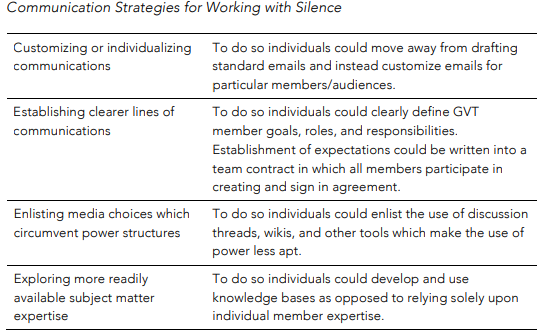
\includegraphics[width=120mm,height=62mm,scale=1]{TAS/Images/CommunicationStrategies.png}\\
\end{center}
The above approach mentions incorporating information and communication technologies that address members’ communication needs and circumvent biases. For example, one could develop discussion boards to
facilitate equality of input on the part of all members. An understanding of the task will facilitate the negotiation of availability and exchange of information critical to success. 

\subsection{Meeting Policies and Guidelines}
Several studies advocate for the implementation of explicit meeting policies and guidelines. A comprehensive review by Raphaela Brandner through 10 Meeting Rules to Host Productive and Effective Meetings ~\cite{15} analyzed the effects of instituting policies related to meeting frequency, duration, and necessity. Organizations that established clear guidelines experienced a notable decrease in unnecessary meetings, leading to improvements in overall productivity and employee satisfaction.

\subsection{Employee Perspectives and Feedback}
Understanding the perceptions of employees regarding meetings is crucial. A qualitative study by Maureen L. Mackenzie. (2010) ~\cite{16} seeks to uncover the expectations that have yet to be clearly defined within the manager–employee relationship. By delving into the shifting dynamics of communication and trust within this digital framework, the intended outcome is to reveal the uncharted territory and expectations that characterize the evolving relationship between managers and employees in the digital age.

\subsection{Implementation Strategies}
To cut meeting numbers effectively, secure leadership support, with leaders modeling new communication methods. Implement changes gradually for organizational adaptability, fostering a culture where employees readily embrace shifts in meeting practices.

\subsection{Evaluation and Measurement}
Measuring the success of initiatives to reduce meetings is crucial for ongoing improvement. Metrics such as meeting duration, employee satisfaction, and productivity levels are commonly used. Regular evaluations, coupled with feedback mechanisms, enable organizations to refine their strategies and address emerging challenges.

\subsection{Gaps in the Literature}
While existing research provides valuable insights, several gaps remain. Limited studies have explored the long-term effects of reduced meeting frequency on team dynamics and organizational culture. Additionally, more research is needed to understand the cultural nuances that influence meeting behaviors in diverse settings, including universities.
\section{Methodology}
\subsection{How did we approach the problem?}
\begin{enumerate}
{\bfseries \item Eliminate Unnecessary Meetings}: Review the necessity of each meeting and cancel those that are not essential. Consider alternative ways to achieve the meeting's objectives.
{\bfseries \item Set Clear Objectives}: Ensure that every meeting has a clear purpose and defined goals. This will help in keeping the meeting focused and productive. Try out meeting purpose statements ~\cite{17}. Here is an example:
\begin{center}
    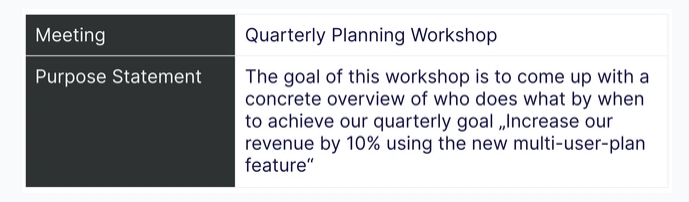
\includegraphics[width=100mm,height=25mm,scale=1]{TAS/Images/Clear-Purpose.png}\\
\end{center}
{\bfseries \item Limit Meeting Frequency}: Assess the necessity of weekly meetings and consider reducing them to biweekly if feasible. Regularly evaluate the need for recurring meetings to avoid unnecessary gatherings.
{\bfseries \item Shorten Meeting Duration}: Strive to keep meetings as short as possible while still achieving their objectives. A one-hour team meeting should be the maximum, and one-on-one meetings can be kept to half an hour.
\end{enumerate}
\subsection{What techniques are used in analysis of results}
\begin{enumerate}
{\bfseries \item Create and Follow Agendas}: Set a formal agenda for every meeting involving more than two people and allocate time to each item listed. Encourage short meetings by moving topics not requiring live discussion to email or other communications.
{\bfseries \item Consider Alternative Meeting Formats}: Explore the use of asynchronous meetings and other communication tools to reduce the need for in-person gatherings.
{\bfseries \item Evaluate Meeting Attendance}: Only invite necessary participants to each meeting and consider scheduling more meetings with fewer attendees to keep them shorter and more focused.
{\bfseries \item Implement Meeting Time Management}: Start meetings on time, end them early whenever possible, and set ground rules to establish norms for behavior and expectations.
{\bfseries \item Document and Follow Up}: Take responsibility for summarizing all decisions and outcomes after each meeting, and document and follow up on all action items generated.
{\bfseries \item Block Out "No Meeting" Times}: Block out specific times during the day as "busy" in your calendar to prevent organizers from scheduling unnecessary meetings.
\end{enumerate}
\subsection{Potential Solutions}
The issue of avoiding too many meetings in work environments is a common challenge, and it's crucial to address it effectively to maintain productivity and employee well-being. Here are some potential solutions and strategies to mitigate the problem:
\begin{enumerate}
{\bfseries \item  Implement Clear Meeting Guidelines}:
Establish clear guidelines on when to schedule meetings and when to use alternative communication channels. Encourage the use of asynchronous communication tools for non-urgent matters.
Define the purpose and agenda for each meeting to ensure that they are focused and efficient.
{\bfseries \item  Encourage Asynchronous Communication}:
Promote the use of collaboration tools that support asynchronous communication, such as project management platforms, chat applications, and document-sharing systems.
Encourage team members to provide updates and information in written form when possible, reducing the need for frequent meetings.
{\bfseries \item  Evaluate Meeting Necessity}:
Introduce a system for evaluating the necessity of each meeting. Require organizers to justify the need for a meeting and assess whether the same objectives can be achieved through other means.
{\bfseries \item  Implement Agile Practices Effectively}:
Ensure that agile practices are implemented in a way that aligns with the remote work environment. This may involve adapting traditional agile ceremonies to suit virtual collaboration.
Explore virtual alternatives for agile practices, such as online retrospectives, sprint planning, and daily stand-ups.
{\bfseries \item  Limit Meeting Duration and Size}:
Set guidelines for meeting duration and the number of participants. Encourage shorter, more focused meetings to prevent unnecessary time consumption.
Consider breaking down large meetings into smaller, more targeted sessions to maintain relevance for all participants.
{\bfseries \item  Educate Teams on Effective Remote Collaboration}:
Provide training on remote collaboration techniques and best practices. This can include guidance on using collaboration tools, managing time effectively in a remote setting, and establishing boundaries between work and personal life.
{\bfseries \item  Regularly Review and Adjust}:
Periodically review the meeting practices and gather feedback from employees. Be willing to adapt and adjust strategies based on the evolving needs and challenges of remote work.
{\bfseries \item  Utilize Technology Wisely}:
Leverage technology to streamline meetings, such as utilizing AI-driven scheduling tools ex: Microsoft's MyAnalytics tool, for instance, tracks workers' email traffic, response time, and time devoted to meetings, attempting to optimize their work routines (setting default meeting lengths, and using features that promote engagement and participation.) ~\cite{08}
{\bfseries \item  Encourage Open Communication}:
Foster an environment where employees feel comfortable expressing concerns about meeting overload. Encourage open communication and collaboration to collectively find solutions.
{\bfseries \item  Empower Organizers to Make Informed Decisions}:
Provide guidelines and training to meeting organizers to help them make informed decisions about the necessity, format, and size of meetings. Encourage them to consider alternative communication methods when appropriate.
\end{enumerate}
By implementing a combination of these strategies, organizations can work towards reducing meeting overload in remote agile settings while maintaining the collaborative and communicative aspects integral to agile methodologies ~\cite{07}.
\section{Lessons Learned}
Optimize meetings by prioritizing agendas, embracing technology, and fostering a culture valuing efficiency, reducing time-wasting practices effectively.
\begin{itemize}
\item Based on the research, it is evident that having too many meetings can lead to decreased productivity, employee disengagement, and a waste of time and money.
\item The common reasons for too many meetings include lack of trust within the team, unclear roles, and the habit of over-scheduling meetings due to these factors.
\item To avoid unnecessary meetings, it is important to set an agenda, consider asynchronous meetings, and use meeting management tools.
\item It is crucial to consider the number of invitees for a meeting, as having too many people can lead to inefficiency and unproductive discussions.
\item It is recommended to decline meeting invitations when possible to reduce the number of meetings during the day or week.
\end{itemize}
\subsection{Quality of the lessons}
The lessons learned are adequate as they are based on research findings and provide actionable strategies for avoiding too many meetings. The information is comprehensive and addresses the reasons for excessive meetings, the ideal cadence for meetings, and practical tips for reducing unnecessary meetings.
\subsection{Under what conditions}
The lessons are applicable in work environments where there is a concern about the negative impact of excessive meetings on productivity and employee well-being. They can be implemented in various organizations and teams to improve the quality and effectiveness of meetings.
\subsection{Constraints}
While the lessons provide valuable insights and strategies, it's important to note that the effectiveness of implementing these recommendations may vary based on the specific organizational culture, team dynamics, and industry norms. Additionally, individual preferences and work styles may influence the success of reducing the number of meetings.
Overall, the lessons learned from the research provide valuable guidance for addressing the issue of too many meetings, and they can serve as a foundation for improving meeting practices in the workplace.
\section{Conclusions And Future Works}
To avoid having too many meetings, it is important to structure meetings effectively and eliminate unnecessary ones. Here are some strategies to achieve this:
\subsection{Building Better Meetings}
\begin{enumerate}
{\bfseries \item Have a clear purpose}: Every meeting should have a specific point and be only as long as necessary to achieve its goals.
{\bfseries \item Regular team meetings}: Schedule team meetings including everyone and one-on-one meetings with each contributor. Test the necessity of weekly meetings and consider rescheduling them to be biweekly if possible.
{\bfseries \item Strive for brevity}: Encourage short meetings by moving topics not requiring live discussion to email or other communications. Set a formal agenda for every meeting involving more than two people and allocate time to each item listed.
{\bfseries \item Consider hijacking regular team meeting agenda for special-purpose meetings}: Dispense with normal team business quickly and move on to the particular topics.
\end{enumerate}
\newpage
\subsection{Running Better Meetings}
\begin{enumerate}
{\bfseries \item Start and end on time}: Start meetings on time and end early whenever possible. Use a 'bucket list' to capture off-topic issues that arise and follow up on all action items generated.
{\bfseries \item Set ground rules}: Establish norms for behavior and set expectations that participants will not be wasting their time.
\end{enumerate}
\subsection{Rationalizing Meetings}
{\bfseries Review and cancel unnecessary meetings}: Before scheduling any meeting, consider if there might be a better way to accomplish the objectives. Review all current meetings and cancel those that are not necessary.
\subsection{Future Work}
\begin{enumerate}

{\bfseries \item Implementation and Testing:}
\begin{itemize}
  \item Develop and implement strategies based on the recommendations from your literature review. This could involve piloting new meeting policies or communication tools in specific departments or teams.
   \item Collect feedback from participants to understand the impact of the changes on their work and overall productivity.
\end{itemize}
{\bfseries \item Technology Integration:}
\begin{itemize}
   \item Explore the integration of specific technologies or tools aimed at reducing the need for meetings. Consider platforms that support asynchronous communication, collaborative document editing, and project management.
   \item Assess the effectiveness of these tools in fostering efficient communication without the necessity for frequent face-to-face meetings.
\end{itemize}
{\bfseries \item Training and Awareness Programs:}
\begin{itemize}
   \item Develop training programs for employees and leaders to enhance meeting effectiveness. This could include workshops on efficient meeting practices, the use of collaborative tools, and time management.
   \item Implement awareness campaigns to promote a cultural shift towards valuing time and reducing unnecessary meetings.
\end{itemize}
{\bfseries \item Continuous Improvement:}
\begin{itemize}
   \item Establish a continuous improvement process for meeting policies and practices. Regularly review and update guidelines based on feedback and changing organizational needs.
   \item Monitor key performance indicators (KPIs) related to meeting efficiency and employee satisfaction to gauge the success of implemented strategies.
\end{itemize}
{\bfseries \item Cultural Shift Initiatives:}
\begin{itemize}
   \item Implement initiatives to foster a cultural shift toward mindful meeting practices. This might involve leadership endorsements, recognition programs for efficient meeting conduct, and incentives for teams that successfully reduce meeting frequency.
   \item Evaluate the impact of these cultural initiatives on the overall meeting culture of the organization.
\end{itemize}
{\bfseries \item Employee Well-being Focus:}
\begin{itemize}
   \item Assess the impact of reduced meeting frequency on employee well-being. Consider conducting surveys or interviews to understand how changes in the meeting culture influence job satisfaction, work-life balance, and stress levels.
   \item Implement wellness programs to support employees in managing their time and workload effectively.
\end{itemize}
{\bfseries \item Benchmarking and Comparative Studies:}
\begin{itemize}
   \item Explore opportunities for benchmarking against other organizations that have successfully reduced meeting frequency.
   \item Conduct comparative studies to understand how different industries or sectors manage their communication and collaboration needs with fewer meetings.
\end{itemize}
{\bfseries \item Long-Term Effects:}
\begin{itemize}
   \item Investigate the long-term effects of reduced meeting frequency on team dynamics, creativity, and innovation.
   \item Examine how the changes influence organizational adaptability and responsiveness in the face of evolving challenges.
\end{itemize}
{\bfseries \item Integration with Remote Work Practices:}
\begin{itemize}
   \item If applicable, explore the intersection of meeting reduction strategies with remote work practices.
   \item Evaluate how a hybrid or fully remote work environment affects the need for meetings and communication strategies.
\end{itemize}
\end{enumerate}
Engaging with stakeholders and continuously gathering feedback will be crucial for the successful implementation and improvement of meeting practices within any organization.


